\documentclass[11pt]{article}
\usepackage[a4paper,margin=1in]{geometry}
\usepackage{amsmath,amssymb,amsthm,mathtools}
\usepackage{booktabs}
\usepackage{enumitem}
\usepackage{graphicx}
\usepackage{microtype}
\usepackage{hyperref}
\usepackage[nameinlink,capitalise]{cleveref}
\usepackage[numbers,sort&compress]{natbib}

\newtheorem{theorem}{Theorem}[section]
\newtheorem{proposition}[theorem]{Proposition}
\newtheorem{corollary}[theorem]{Corollary}
\newtheorem{lemma}[theorem]{Lemma}
\theoremstyle{definition}
\newtheorem{definition}[theorem]{Definition}
\theoremstyle{remark}
\newtheorem{remark}[theorem]{Remark}
\newcommand{\norm}[1]{\left\lVert#1\right\rVert}
\newcommand{\tr}{\operatorname{tr}}
\newcommand{\Ran}{\operatorname{Ran}}
\newcommand{\E}{\mathcal E}

\title{Two-Direction Recursive Ritz Refresh\\
\large An At-Most-Nine-Dimensional Closure of the Four-Step Schur Packet Chain}
\author{Liang Wang}
\date{July 2026}

\begin{document}
\maketitle

\begin{abstract}
RH-92 replaced pointwise sub-quarter decay by a four-step contraction budget,
but refreshed the old packet from an ambient leading eigenspace at every
update.  This paper asks whether the refresh itself can remain recursively
low dimensional.

Let $V$ be a rank-$r$ packet and choose $k$ orthonormal directions
$Q\subset\Ran(I-VV^*)$.  For
\[
 H=[V,Q]^*G[V,Q]=
 \begin{pmatrix}A&B\\B^*&D\end{pmatrix},
\]
retaining the leading $r$ Ritz directions gains exactly
\[
 \Delta_k=\tr D-\sum_{i=1}^k\lambda_i^{\uparrow}(H).
\]
The top-$k$ left singular directions of the projected cross operator
$(I-VV^*)GV$ maximize captured cross Frobenius energy.  For any full-rank
trial frame $W\in\mathbb C^{(r+k)\times k}$, Ky Fan's principle gives the
reference-free certificate
\[
 \tr\!\left((W^*W)^{-1}W^*HW\right)+\delta\le\tr D
 \quad\Longrightarrow\quad \Delta_k\ge\delta.
\]
This formulation is invariant under a nonorthonormal numerical frame.

We then use the corrected Ritz packet itself as the next packet, with no
ambient refresh inside the block.  A 384-bit audit compares one, two, and
three projected-cross directions over the ten RH-92 windows.  The recursive
one-direction block has geometric mean above $0.24$ in four fine channels,
reaching $0.32213305$.  Two directions reverse all four failures: all forty
two-frame forms are strictly negative, every exact rational block budget is
below $0.24^4$, and the largest direct block geometric mean is
$0.22850222$.  The top two directions capture at least $96.376\%$ of the
projected-cross energy, and the compressed dimension is at most nine.  Three
directions reduce the worst endpoint tail/reference-tail ratio to $1.05595$.

Thus the ambient in-block packet reset is removed from the frozen
certificate, and the second direction is genuinely necessary there.  No
uniform all-level two-direction law, continuum cross-direction construction,
Stage-A closure, Hilbert--Polya operator, or Riemann Hypothesis result is
claimed.
\end{abstract}

\noindent\textbf{Keywords:} Rayleigh--Ritz; recursive packet; Ky Fan
principle; cross Gramian; reduced refresh; validated numerics.

\medskip
\noindent\textbf{MSC 2020:} 47A75; 15A18; 65F15; 65G20; 37C30.

\section{Introduction}

The late-memory packet route has progressively reduced an ambient
effective-rank question to small variational objects.  RH-89 showed that one
complement direction gives a strong isolated Ritz correction
\citep{WangRitz2026}.  RH-90 converted its required gain into a Schur trial
sign \citep{WangSchur2026}.  RH-91 extracted a conditional tail bootstrap
\citep{WangPacketReview2026}, and RH-92 weakened the overly rigid pointwise
target to a four-step product budget \citep{WangBlockBudget2026}.

One structural gap remained visible in RH-92.  At every update, its old
packet was recomputed as the leading rank-$r$ packet of the new ambient
Gramian.  The rank-one Ritz packet certified the local energy gain but was not
itself carried into the next update.  Consequently the finite certificate
still used an ambient spectral refresh between two small Schur solves.  This
was exactly why the revised Stage-A frontier kept the Schur block gate and
the reduced-refresh gate separate.

The present paper tests the most economical way to remove that reset.  Start
with one leading seed packet at the beginning of the four-step window.  At
each later update:

\begin{enumerate}[leftmargin=2em]
\item apply the new Gramian to the current packet and project away the packet;
\item retain the first $k$ left singular directions of this projected cross
operator;
\item solve one $(r+k)$-dimensional Ritz problem;
\item use its leading rank-$r$ packet as the input to the next update.
\end{enumerate}

No ambient eigenspace is inserted inside the chain.  The projected cross
operator has only $r$ columns, so its nonzero singular data can be found from
an $r\times r$ Gram matrix after applying $G$ to the current packet.  The
remaining spectral solve has dimension $r+k$.

There are three mathematical tasks.  First, the rank-one gain identity must
be extended to arbitrary complement width $k$.  Second, the complement
directions need a canonical optimality statement.  Third, the scalar Schur
trial must be replaced by a $k$-frame certificate that remains valid for an
almost orthonormal numerical frame.  These are supplied in
\cref{sec:theory,sec:frame}.

The numerical conclusion is unusually sharp.  Width one is not merely less
accurate: its recursive block target fails in all four channels at
$\sigma=0.02$ and $0.01$.  Width two passes all ten channels.  Width three is
not needed for contraction, but nearly reproduces the endpoint leading
packet in every channel.  This gives a genuine finite threshold between one
and two directions while separating target sufficiency from near-optimal
tracking.

\section{Multi-direction complement Ritz refresh}
\label{sec:theory}

Let $G=G^*\ge0$ act on a finite-dimensional Hilbert space $\mathcal K$.
Let $V:\mathbb C^r\to\mathcal K$ and
$Q:\mathbb C^k\to\mathcal K$ be isometries with $V^*Q=0$.  Put
$Z=[V,Q]$ and partition
\begin{equation}
 H=Z^*GZ=
 \begin{pmatrix}A&B\\B^*&D\end{pmatrix},
 \qquad A\in\mathbb C^{r\times r},\quad D\in\mathbb C^{k\times k}.
 \label{eq:block}
\end{equation}
Write the eigenvalues of $H$ in increasing order as
$\lambda_1^\uparrow(H)\le\cdots\le\lambda_{r+k}^\uparrow(H)$.

\begin{theorem}[$k$-direction complement Ritz theorem]
\label{thm:k-ritz}
Let $C$ contain the leading $r$ orthonormal eigenvectors of $H$ and put
$U=ZC$.  Then
\begin{align}
 \tr(U^*GU)
 &=\tr H-\sum_{i=1}^k\lambda_i^\uparrow(H),
 \label{eq:captured}\\
 \Delta_k
 &:=\tr(U^*GU)-\tr(V^*GV)
 =\tr D-\sum_{i=1}^k\lambda_i^\uparrow(H)\ge0.
 \label{eq:gain}
\end{align}
Consequently
\begin{equation}
 E_r(G)\le \E_G(U)\le\E_G(V),
 \qquad
 \E_G(W)=\tr G-\tr(W^*GW)
 \label{eq:tail-order}
\end{equation}
for isometric packets.
\end{theorem}

\begin{proof}
The leading rank-$r$ Ritz capture is the sum of the largest $r$ eigenvalues
of $H$, which equals the right side of \eqref{eq:captured}.  Since
$\tr H=\tr A+\tr D$ and the old coordinate packet captures $\tr A$,
subtraction gives \eqref{eq:gain}.  The old packet range is an admissible
rank-$r$ subspace of $\Ran Z$, so Ky Fan's maximum principle gives
$\Delta_k\ge0$.  The full leading packet can only capture more energy than a
Ritz packet restricted to $\Ran Z$ \citep{Fan1949,Bhatia1997}.
\end{proof}

For $P=VV^*$, define the projected cross operator
\begin{equation}
 K=(I-P)GV:\mathbb C^r\longrightarrow\Ran(I-P).
 \label{eq:cross}
\end{equation}
It can be formed without constructing a basis for the full complement:
$K=GV-V(V^*GV)$.

\begin{proposition}[Top-$k$ projected-cross selection]
\label{prop:cross}
Let $s_1(K)\ge s_2(K)\ge\cdots$ be the singular values of $K$.  Among all
isometries $Q:\mathbb C^k\to\Ran(I-P)$,
\begin{equation}
 \max_Q\norm{Q^*GV}_{S_2}^2
 =\sum_{i=1}^k s_i(K)^2.
 \label{eq:cross-max}
\end{equation}
The maximizing range is spanned by the first $k$ left singular vectors of
$K$, and for this choice
\begin{equation}
 \norm{(I-QQ^*)K}_{S_2}^2=\sum_{i>k}s_i(K)^2.
 \label{eq:cross-tail}
\end{equation}
\end{proposition}

\begin{proof}
Since $Q^*V=0$, $Q^*GV=Q^*K$.  Ky Fan's maximum principle applied to
$KK^*$ proves \eqref{eq:cross-max}; the singular-value expansion then gives
\eqref{eq:cross-tail} \citep{GolubVanLoan2013}.
\end{proof}

This proposition does not by itself bound the corrected packet tail.  It
identifies the canonical $k$-dimensional part of the cross interaction.  The
complement diagonal block $D$ and the joint Ritz rotation still matter.  The
audit therefore records cross-energy capture as a mechanism diagnostic, not
as a substitute for the final gain certificate.

\begin{corollary}[Nested enrichment monotonicity]
\label{cor:nested}
If the selected complement spaces are nested,
$\Ran Q_k\subset\Ran Q_{k+1}$, then the restricted optimal tail is
nonincreasing in $k$ at one fixed update.
\end{corollary}

\begin{proof}
The rank-$r$ trial spaces available in $\Ran[V,Q_k]$ form a nested family.
Apply the variational principle.
\end{proof}

The corollary is one-step only.  Recursive width-$k$ chains follow different
packets after the first update, so their later comparison is not a formal
consequence of nesting.

\section{Generalized trial-frame gain certificate}
\label{sec:frame}

The gain in \eqref{eq:gain} is controlled by the sum of the bottom $k$
eigenvalues of $H$.  A $k$-dimensional analogue of the RH-90 trial vector is
therefore a trial frame for the bottom spectral subspace.

For any full-column-rank
$W\in\mathbb C^{(r+k)\times k}$, define its generalized Rayleigh trace
\begin{equation}
 \mathcal R_H(W)
 =\tr\!\left((W^*W)^{-1}W^*HW\right).
 \label{eq:generalized-trace}
\end{equation}
This quantity depends only on $\Ran W$, not on the chosen frame coordinates.

\begin{theorem}[Generalized trial-frame gain certificate]
\label{thm:frame}
For every full-rank trial frame $W$,
\begin{equation}
 \sum_{i=1}^k\lambda_i^\uparrow(H)
 \le\mathcal R_H(W).
 \label{eq:frame-upper}
\end{equation}
Hence, for any requested gain $\delta\ge0$,
\begin{equation}
 \boxed{
 \Psi_{\delta,k}(W)
 :=\mathcal R_H(W)+\delta-\tr D\le0
 \quad\Longrightarrow\quad
 \Delta_k\ge\delta.}
 \label{eq:frame-certificate}
\end{equation}
\end{theorem}

\begin{proof}
Let $M=W^*W\succ0$ and set $Y=WM^{-1/2}$.  Then $Y^*Y=I_k$, and cyclicity
of the trace gives
\[
 \tr(Y^*HY)=\tr(M^{-1}W^*HW)=\mathcal R_H(W).
\]
Ky Fan's minimum principle identifies the sum of the bottom $k$ eigenvalues
as the minimum of this trace over all orthonormal $k$-frames.  This proves
\eqref{eq:frame-upper}.  Combine it with \eqref{eq:gain}.
\end{proof}

The metric factor $(W^*W)^{-1}$ makes the certificate exactly invariant under
a nonorthonormal floating frame.  No post hoc assumption that the computed
eigenvectors are exactly orthogonal is needed.  For $k=2$, the metric inverse
is evaluated by its explicit $2\times2$ determinant in the interval audit.

\begin{theorem}[Recursive reduced block closure]
\label{thm:recursive}
Let $G_j\ge0$ be a sequence of Gramians.  Start with an isometric rank-$r$
packet $V_{b}$.  At update $j>b$, construct $k$ projected-cross directions,
form the enriched compression, and let $V_j$ be its leading rank-$r$ Ritz
packet.  Define
\begin{align}
 E_{j-1}&=\E_{G_{j-1}}(V_{j-1}),\\
 C_j&=\E_{G_j}(V_{j-1}),\\
 \delta_j&=C_j-\rho_jE_{j-1},\qquad \rho_j\ge0.
\end{align}
If either $\delta_j\le0$ or a trial frame satisfies
$\Psi_{\delta_j,k}(W_j)\le0$, then
\begin{equation}
 E_j:=\E_{G_j}(V_j)\le\rho_jE_{j-1}.
 \label{eq:recursive-step}
\end{equation}
Consequently, over $m$ recursive updates,
\begin{equation}
 E_{b+m}\le\left(\prod_{j=b+1}^{b+m}\rho_j\right)E_b.
 \label{eq:recursive-product}
\end{equation}
No ambient packet refresh occurs between the updates.
\end{theorem}

\begin{proof}
If $\delta_j\le0$, the old packet already has new tail
$C_j\le\rho_jE_{j-1}$, and Ritz optimization can only improve it.  Otherwise
\cref{thm:frame} gives $\Delta_k\ge\delta_j$.  By
\cref{thm:k-ritz}, the corrected tail is
$C_j-\Delta_k\le C_j-\delta_j=\rho_jE_{j-1}$.  Iteration proves
\eqref{eq:recursive-product}.
\end{proof}

This theorem merges local correction and refresh: the output packet is the
next input packet.  It still requires one seed packet and a uniform method for
constructing the projected-cross directions.

\section{384-bit recursive audit}

\subsection{Models and block protocol}

We use the five frozen Gaussian scales
$\sigma=0.16,0.08,0.04,0.02,0.01$, two directional channels per scale,
$\eta=1/512$, and clock ranks $4,5,6,6,7$.  The four-step windows are the
same as RH-92: $1$--$4$, $3$--$6$, $8$--$11$, $14$--$17$, and $19$--$22$.

Each chain is seeded once by the leading packet at the time immediately
before the block.  Thereafter width one, two, or three is propagated
recursively.  The two-direction chain is the primary certificate.  The
one-direction chain is a negative comparator, and width three measures how
closely a slightly larger packet tracks the endpoint leading reference.
The reference packet is not inserted into any recursive chain.

At a primary update, the implementation forms
\[
 K_j=G_jV_{j-1}-V_{j-1}(V_{j-1}^*G_jV_{j-1}),
\]
extracts its first two left singular vectors, and solves an
$(r+2)$-dimensional Ritz problem.  The largest primary compression is
$9\times9$.

\subsection{Exact-binary validation layers}

The binary64 pilot selects upward-rounded thousandth budgets, which are then
frozen as exact rational numbers.  The 384-bit audit checks:

\begin{enumerate}[leftmargin=2em]
\item the generalized two-frame form in \eqref{eq:frame-certificate};
\item the direct recursive tail ratio for each update;
\item the exact four-step endpoint/seed tail ratio;
\item positivity of the $2\times2$ frame metric determinant;
\item orthogonality defects of the enriched and corrected packets.
\end{enumerate}

As in RH-92, ambient residuals use the metric-corrected expression
\begin{equation}
 \E_G(W)=\tr G-2\tr(W^*GW)
 +\tr\bigl((W^*W)(W^*GW)\bigr),
 \label{eq:metric-tail}
\end{equation}
which is valid for the exactly lifted binary basis.  Compressed frame forms
and ambient recursive tails are therefore certified separately.  This is the
same distinction between a small variational model and its floating ambient
realization used in validated numerical linear algebra
\citep{Higham2002,Rump2010}.

\section{Results: one direction fails, two directions close}

\begin{table}[ht]
\centering
\scriptsize
\begin{tabular}{rrrllrrrr}
\toprule
$\sigma$ & side & rank & times & two-direction budgets & one mean & two mean & min cross-2 & three/ref\\
\midrule
0.16 & L & 4 & 1--4 & .007/.005/.004/.003 & .015121 & .004011 & .999380 & 1.000001\\
0.16 & R & 4 & 1--4 & .011/.006/.003/.003 & .020379 & .004200 & .999982 & 1.000006\\
0.08 & L & 5 & 3--6 & .012/.006/.007/.017 & .037582 & .008976 & .999989 & 1.000461\\
0.08 & R & 5 & 3--6 & .008/.039/.003/.021 & .053466 & .010914 & .999958 & 1.007250\\
0.04 & L & 6 & 8--11 & .079/.081/.056/.026 & .105841 & .054339 & .999999 & 1.000220\\
0.04 & R & 6 & 8--11 & .036/.065/.180/.089 & .091346 & .077737 & .999999 & 1.055945\\
0.02 & L & 6 & 14--17 & .455/.145/.120/.233 & .270599 & .206639 & .963762 & 1.000529\\
0.02 & R & 6 & 14--17 & .137/.256/.356/.113 & .315010 & .193248 & .995872 & 1.000578\\
0.01 & L & 7 & 19--22 & .335/.248/.168/.197 & .316481 & .228502 & .990854 & 1.001758\\
0.01 & R & 7 & 19--22 & .343/.250/.123/.153 & .322133 & .199990 & .999704 & 1.005420\\
\bottomrule
\end{tabular}
\caption{Recursive packet results.  Means are fourth roots of interval block
ratios.  ``Min cross-2'' is the smallest top-two projected-cross energy
fraction in the channel.  ``Three/ref'' is the endpoint width-three tail
divided by the endpoint leading-packet tail.}
\label{tab:channels}
\end{table}

The one-direction failures are exactly the four fine channels at
$\sigma=0.02$ and $0.01$.  Their geometric means are rigorously above $0.24$.
The largest is $0.32213305$.  Thus the RH-89/RH-90 one-direction correction,
although strong when restarted from a leading packet, does not recursively
carry its own packet through these four windows.

Two directions close all ten blocks.  The hardest rational budget is the
left channel at $\sigma=0.01$:
\[
 0.335\cdot0.248\cdot0.168\cdot0.197
 =0.00274961568
 =0.82875666\cdot0.24^4.
\]
Its direct interval geometric mean is at most $0.22850222$.  The largest
individual two-direction contraction is $0.45462724$, so the success remains
a block phenomenon rather than a pointwise sub-quarter law.

\begin{table}[ht]
\centering
\small
\begin{tabular}{lr}
\toprule
validated quantity & worst certified value\\
\midrule
generalized two-frame signs & 40/40 strict\\
direct two-direction target contractions & 40/40\\
one-direction failed blocks & 4/10\\
two-direction green blocks & 10/10\\
largest one-direction block mean & $0.32213305$\\
largest two-direction budget mean & $0.22899079$\\
largest two-direction direct mean & $0.22850222$\\
largest three-direction direct mean & $0.22620607$\\
minimum top-one cross-energy fraction & $0.586156$\\
minimum top-two cross-energy fraction & $0.963762$\\
smallest negative two-frame margin & $6.2621\times10^{-18}$\\
largest primary compressed dimension & $9$\\
largest two-direction endpoint/reference ratio & $15.916$\\
largest three-direction endpoint/reference ratio & $1.05595$\\
\bottomrule
\end{tabular}
\caption{Global 384-bit summary.  The endpoint/reference ratio is a tracking
diagnostic, not part of the contraction certificate.}
\label{tab:summary}
\end{table}

The cross-energy diagnostic explains why the second direction matters.  At
the hardest update the leading cross direction captures only $58.616\%$ of
the projected-cross Frobenius energy, whereas the first two capture
$96.376\%$.  Across most other updates the top-two fraction is above
$99.9\%$.

Two directions are sufficient for the target but not uniformly
near-optimal.  In the coarse right channel at $\sigma=0.08$, its endpoint tail
is about $15.9$ times the very small leading-packet tail, even though its
four-step contraction is excellent.  Width three reduces the worst such
ratio over all channels to $1.05595$.  This distinction is useful: a theorem
aimed only at the Stage-A residual may prefer width two, while a theorem that
needs stable packet identification may pay for a third direction.

\begin{figure}[ht]
\centering
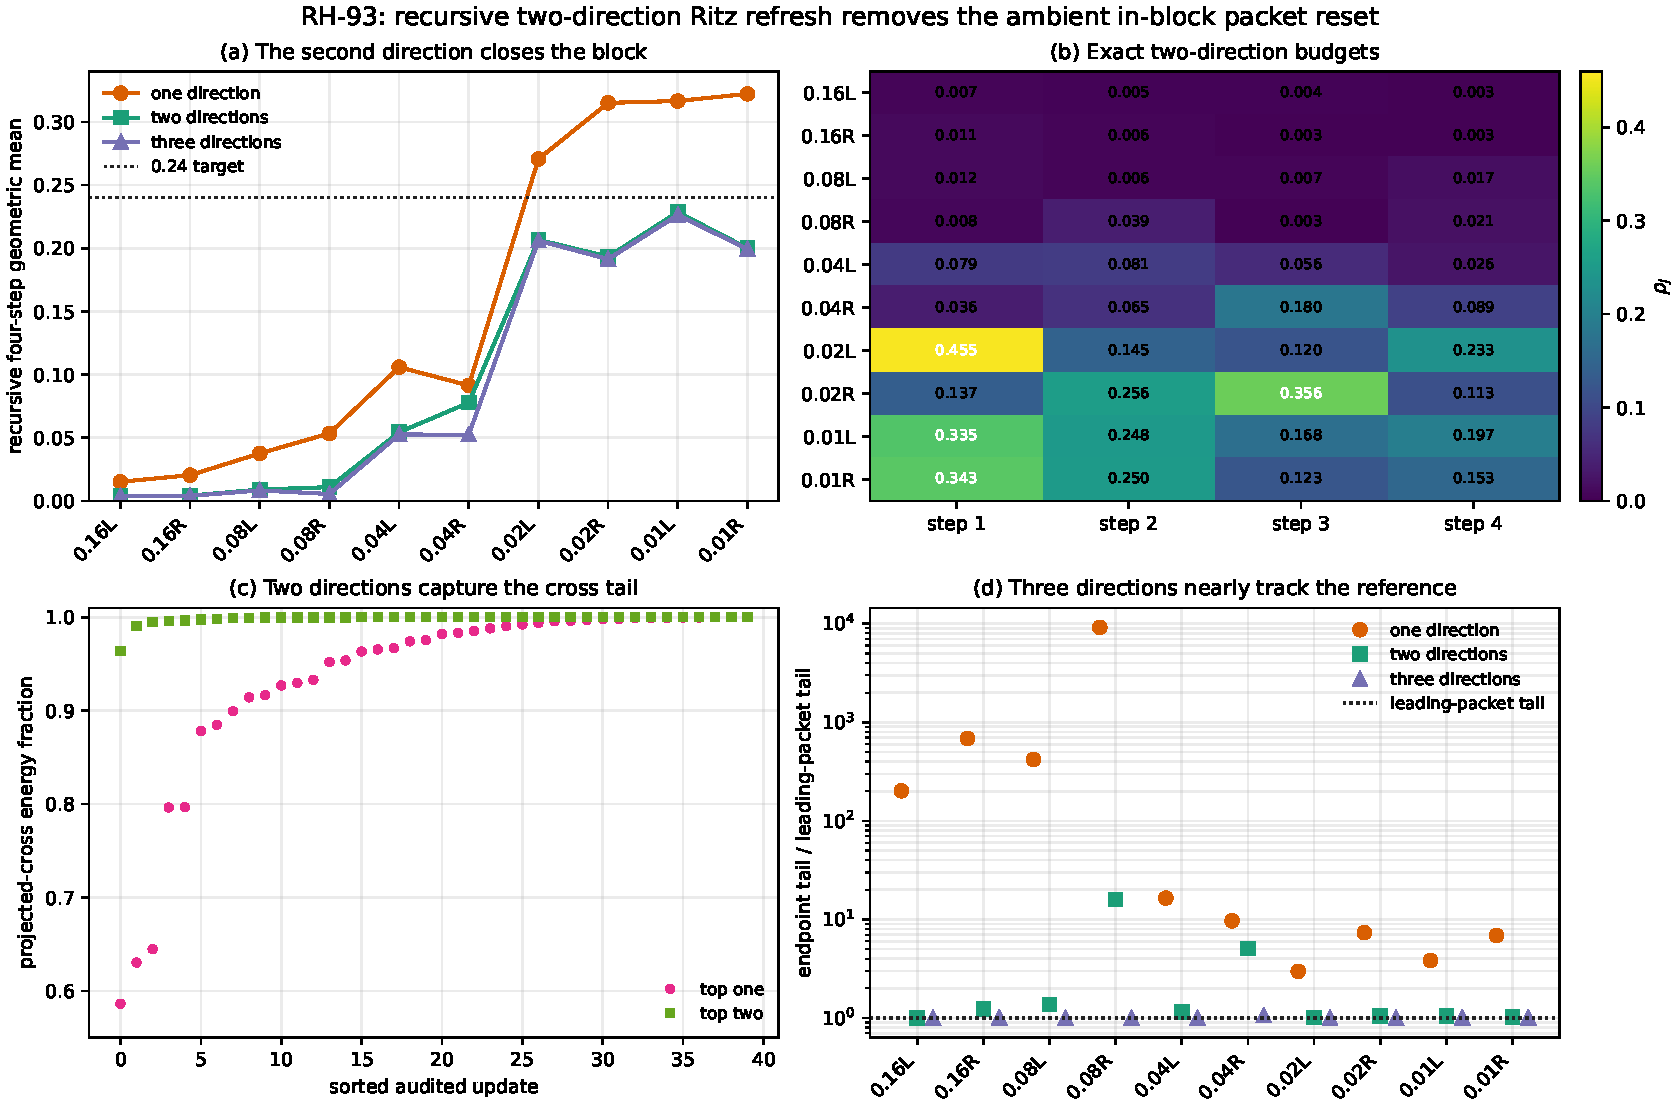
\includegraphics[width=\textwidth]{figures/two_direction_recursive_ritz_refresh.pdf}
\caption{Recursive complement width.  Panel (a) shows the four fine failures
of width one and universal width-two closure.  Panel (b) displays the exact
rational two-direction budgets.  Panel (c) compares top-one and top-two
projected-cross energy capture.  Panel (d) shows endpoint tracking relative
to the ambient leading packet; width three is uniformly close at the stored
anchors.}
\label{fig:audit}
\end{figure}

\section{Revised frontier and limitations}

RH-92 expressed the preferred Stage-A corridor as a block Schur law
$S_{\mathrm{blk}}$, a reduced refresh/future gate $R$, and the inherited
prefix/normalization/observability bridge $O$.  The present recursive theorem
suggests a more economical combined gate:
\[
 \begin{aligned}
 D_2:\quad &\text{a uniform two-direction projected-cross Ritz chain}\\
            &\text{with a contracting fixed-length block product}.
 \end{aligned}
\]
If $D_2$ is proved all-level, the sufficient frontier becomes
\begin{equation}
 \mathsf A_1=L\ \vee\ (D_2\wedge O),
 \label{eq:frontier}
\end{equation}
where $L$ is the inherited full-block corridor.  In this formulation $D_2$
supplies both the block contraction and the in-block reduced refresh.

The finite result does not prove $D_2$.  Its remaining components are
explicit:

\begin{itemize}[leftmargin=2em]
\item construct the initial seed packet uniformly at the clock rank;
\item control the first two singular directions of $(I-P)GP$ without frozen
binary models;
\item prove a repeated block product below one after a uniform burn-in;
\item propagate the resulting packet through the physical future with the
normalization and observability factors in $O$.
\end{itemize}

The ambient leading eigensolve is removed only \emph{inside} the frozen
four-step block.  Applying $G$ to the current rank-$r$ packet remains an
ambient operation, though its singular analysis is only $r$-column and its
spectral solves are at most nine dimensional.  No complexity theorem or
continuum limit for those actions is proved.

The one-direction failure is branch-specific.  A different rank staircase,
block phase, or complement selector may repair it.  Conversely, the
three-direction near-reference observation is finite evidence, not a uniform
subspace theorem.

The RH-81 moving-cloud projection, coefficient bridge, and uniform
trace-class complement are unchanged \citep{WangRouteReview2026}.  This paper
constructs no canonical scattering completion, self-adjoint generator,
intrinsic $T\log T$ law, prime-power trace formula, completed-zeta identity,
Hilbert--Polya operator, zeta-zero identification, or proof of the Riemann
Hypothesis.

\section{Reproducibility}

The archive contains the full and smoke audits, the frozen rational budgets,
all forty generalized frame forms, exact-binary recursive residuals for
widths one through three, cross singular-value diagnostics, generated figures,
unit tests, and SHA-256 manifests for local sources, dependencies, and
publication artifacts.  The accompanying README lists the reproduction
commands.  Every interval sign and tail ratio is evaluated after exact binary
lifting at 384-bit precision.

\bibliographystyle{plainnat}
\bibliography{references}

\end{document}
